\documentclass[11pt, letterpaper]{article}

% Paquetes de codificación y lenguaje
\usepackage[utf8]{inputenc}
\usepackage[spanish,mexico]{babel}

% Paquete de Geometría para márgenes profesionales (headheight ajustado para evitar warnings)
\usepackage[margin=2.5cm, headheight=15pt]{geometry}

% Definición de Identidad Institucional y colores para tablas
\usepackage[table]{xcolor}
\definecolor{AzulUNAM}{HTML}{002B5C}
\definecolor{OroUNAM}{HTML}{D4AF37}
\definecolor{GrisFondo}{HTML}{F8F9FA} % Gris muy tenue para cajas y tablas
\definecolor{GrisTabla}{HTML}{E9ECEF}

% Paquetes para tipografía premium y justificación perfecta
\usepackage{palatino} % Fuente serif muy profesional y elegante
\usepackage{microtype} % Mejora el espaciado y evita palabras cortadas extrañas
\usepackage{amsmath}
\usepackage{amsfonts}

% Paquetes para tablas profesionales
\usepackage{booktabs}
\usepackage{multirow}
\usepackage{tabularx}

% Paquete para cajas de texto estilizadas (Banners y Entrevista)
\usepackage{tcolorbox}
\tcbuselibrary{skins, breakable}

% Paquete de personalización de títulos
\usepackage{titlesec}
\titleformat{\section}
  {\normalfont\Large\bfseries\color{AzulUNAM}}{\thesection.}{1em}{}[\vspace{0.2ex}{\color{OroUNAM}\titlerule[1pt]}]
\titleformat{\subsection}
  {\normalfont\large\bfseries\color{AzulUNAM}}{\thesubsection.}{1em}{}

% Paquete para encabezados y pies de página
\usepackage{fancyhdr}
\pagestyle{fancy}
\fancyhf{}
\fancyhead[L]{\textcolor{AzulUNAM}{\textbf{Redes de Datos Seguras}}}
\fancyhead[R]{\textcolor{AzulUNAM}{Facultad de Ingeniería, UNAM}}
\fancyfoot[C]{\thepage}
\renewcommand{\headrulewidth}{1.5pt}
\renewcommand{\headrule}{\hbox to\headwidth{\color{OroUNAM}\leaders\hrule height \headrulewidth\hfill}}

% Paquete de interactividad (Enlaces discretos)
\usepackage[hidelinks, colorlinks=true, linkcolor=AzulUNAM, urlcolor=AzulUNAM, citecolor=AzulUNAM]{hyperref}

\begin{document}

% ================= PORTADA =================
\begin{titlepage}
    \centering
    \vspace*{1.5cm}
    
    % Logo simulado con tipografía
    {\huge \textbf{\textcolor{AzulUNAM}{Universidad Nacional Autónoma de México}}}\\[1cm]
    {\LARGE \textbf{\textcolor{OroUNAM}{Facultad de Ingeniería}}}\\[1.5cm]
    
    % Caja de título principal
    \begin{tcolorbox}[enhanced, colback=AzulUNAM, colframe=AzulUNAM, arc=2mm, 
                      boxrule=0pt, drop fuzzy shadow, top=1cm, bottom=1cm]
        \centering
        {\huge \textbf{\textcolor{white}{Proyecto de Rediseño}}}\\[0.3cm]
        {\LARGE \textbf{\textcolor{OroUNAM}{Instituto de Geografía}}}
    \end{tcolorbox}
    \vspace{1.5cm}
    
    {\Large \textbf{Asignatura:}}\\\vspace{0.2cm}
    {\large Redes de Datos Seguras}\\[1.5cm]
    
    {\Large \textbf{Grupo 8 - Integrantes:}}\\\vspace{0.3cm}
    {\large 
    \begin{tabular}{c}
         Antonio Salgado Octavio Gael \\
         Varela Jimenez Diego \\
         Velasco García Santiago 
    \end{tabular}
    }\\[2cm]
    

    
\end{titlepage}

% ================= ÍNDICE =================
\tableofcontents
\newpage

% ================= CONTENIDO =================

\section{Introducción}
El presente documento técnico expone la planeación, optimización y rediseño de la red cableada interna correspondiente al Edificio Principal del Instituto de Geografía de la UNAM. El diseño de la red aborda de manera integral los aspectos físicos (vías de canalización y cableado estructurado) y lógicos (direccionamiento, VLSM y protocolos), aplicando los conceptos de la asignatura \textit{Redes de Datos Seguras}.

La justificación recae en la necesidad de proveer conectividad robusta a las zonas de investigadores y becarios, respetando las restricciones de infraestructura arquitectónica (como terrazas y zonas de no-cableado) y enlazando los Cuartos de Telecomunicaciones (IDF) con el Cuarto Principal (MDF) mediante tecnología de fibra óptica ligada al anillo principal de la UNAM.

\section{Estudio de campo}

Como parte de la metodología de diagnóstico, se llevó a cabo una entrevista de levantamiento de requerimientos con el equipo de administración de red de la dependencia. Se determinó que las políticas de uso y estándares exigen una modernización a la Categoría 6A para el cableado horizontal, garantizando la transmisión de 10 Gbps para satisfacer la demanda de las "peceras" de becarios y cubículos de investigadores. Se detectaron 54 nodos críticos a recablear y se constató la necesidad de unificar los servicios de voz y datos mediante tecnología VoIP, eliminando el cableado telefónico análogo independiente.

\subsection{Entrevista de Levantamiento Institucional}

Como parte de la fase de recolección de información y comprensión operativa, se llevó a cabo una entrevista presencial con el administrador de la red para entender los estándares, políticas de uso y esquemas de mantenimiento.

% Caja elegante para la entrevista
\vspace{0.5cm}
\begin{tcolorbox}[enhanced, breakable, colback=GrisFondo, colframe=AzulUNAM, 
                  title=\textbf{Transcripción de la Entrevista}, arc=2mm, 
                  boxrule=1pt, attach boxed title to top left={xshift=5mm, yshift=-3mm},
                  boxed title style={colback=AzulUNAM}]
\begin{description}
    \item[\textcolor{AzulUNAM}{Estudiante:}] —¿Qué normativas internacionales siguen para el diseño de la instalación del cableado físico de la red?
    \item[\textcolor{black!70!white}{Profesor:}] —Pues se utiliza cableado estructurado con las normas de la ANSI/TIA, utilizando comúnmente la 606-A y todo lo que corresponde. Porque, si ustedes recuerdan cuando vinieron a la visita, les dije que había cable Cat 5e, Cat 6 y Cat 7.
    \item[\textcolor{AzulUNAM}{Estudiante:}] —¿Cuáles serían las principales políticas de seguridad y control de acceso para los usuarios y dispositivos que residen aquí?
    \item[\textcolor{black!70!white}{Profesor:}] —Pues la seguridad realmente está basada más localmente en los servidores para que no haya intrusiones y, desde luego, para que no entren a los equipos activos en los switches o en los routers. Pero en cuanto a políticas generales, no hay un firewall perimetral porque, por ejemplo, si yo quisiera restringirles el Facebook, tendría problemas porque va a haber quien brinque y diga: \textit{"No, pues yo sí lo ocupo"}.
    \item[\textcolor{AzulUNAM}{Estudiante:}] —Y sobre la administración, ¿cómo segmentan lógicamente la red y qué herramientas utilizan para poder monitorear su estado diariamente?
    \item[\textcolor{black!70!white}{Profesor:}] —Herramienta como tal no existe ninguna; lo que hacemos es directamente a través de la configuración en los equipos, se hacen las VLANs que dividen las redes y así yo puedo segmentar todos los pisos y a todos. Y en cuanto a qué tenemos para monitorear, está el proyecto que se hizo de SNMP, que es lo más básico. Pero si ya lo queremos hacer de una manera más profesional, también está un software que se llama NetSight y otro que se llama Scrutinizer, que son los que permiten hacer más cool los monitoreos.
    \item[\textcolor{AzulUNAM}{Estudiante:}] —Perfecto. Y, por último, en cuanto al mantenimiento: ¿Cada cuánto tiempo y de qué manera realizan el mantenimiento preventivo y correctivo a los equipos y cuartos de telecomunicaciones?
    \item[\textcolor{black!70!white}{Profesor:}] —El mantenimiento preventivo se trata de hacer todo el tiempo, para evitar un problema antes de que suceda. Comúnmente se limpian los equipos y se están depurando las configuraciones. Cada seis meses se apaga el equipo, se sopletea y todo, justo para evitar que vaya a fallar algún componente. Casi siempre es preventivo y procuramos que no haya correctivos.
\end{description}
\end{tcolorbox}
\vspace{0.5cm}

\noindent\textbf{Análisis Técnico de la Entrevista:} \\
La infraestructura actual se apoya firmemente en el estándar de administración ANSI/TIA-606-A, demostrando un nivel de organización en la coexistencia de múltiples categorías de cable. En el ámbito de la seguridad, se opera bajo una filosofía de red abierta en el perímetro (sin firewall), recayendo la mitigación de intrusiones a nivel de host/servidor y aislando los equipos activos. Lógicamente, la segmentación y orden se mantiene mediante la implementación de VLANs configuradas directamente en el hardware de red (Switches y Routers). La visibilidad del estado de la red se gestiona mediante SNMP y herramientas analíticas como NetSight y Scrutinizer. Finalmente, la confiabilidad se sostiene gracias a políticas de mantenimiento semestral preventivo físico, priorizando la vida útil de los componentes y evitando ventanas de mantenimiento correctivas severas.

% ================= SEPARADOR EDIFICIO PRINCIPAL =================
\vspace{1cm}
\begin{tcolorbox}[enhanced, colback=AzulUNAM, colframe=AzulUNAM, arc=0mm, 
                  halign=center, valign=center, top=4mm, bottom=4mm]
    \LARGE\bfseries\color{white} FASE I: EDIFICIO PRINCIPAL
\end{tcolorbox}
\addcontentsline{toc}{section}{Fase I: Edificio Principal}
\vspace{0.5cm}

\section{Marco teórico}

\subsection{Fenomenología Electromagnética y Normativa de Canalización}
Los medios de transmisión guiados sufren alteraciones electromagnéticas durante su recorrido, tales como atenuación, distorsión por retardo y diafonía (NEXT, FEXT). Para mitigar estas mermas en la banda ancha, el cableado UTP Categoría 6A utiliza un trenzado optimizado de 4 pares (23 AWG). La canalización debe respetar la norma ANSI/TIA-569-B, evitando el paralelismo cercano con líneas eléctricas de alta tensión y respetando las capacidades máximas de llenado para evitar tensiones mecánicas que degraden la certificación del enlace.

\subsection{Cálculo Analítico de Capacidad de Llenado para UTP Cat 6A}
De acuerdo con el análisis planimétrico de la Planta Baja, se deben enrutar cables a través de una longitud de 30 metros. Considerando la tasa de llenado sugerida (40\% al 60\%) para evitar deformaciones en la chaqueta del cable, tenemos el siguiente cálculo analítico para 120 servicios teóricos simultáneos usando un diámetro estándar de Categoría 6A:

\begin{equation}
    \text{Capacidad máxima (Cat 6A)} = 76 \text{ cables por canaleta (al 60\% de llenado)}
\end{equation}
\begin{equation}
    \text{Número de canaletas} = \frac{120 \text{ cables}}{76 \text{ cables/canaleta}} \approx 1.57 \implies \mathbf{2 \text{ canaletas}}
\end{equation}

Para cubrir 30 metros de longitud con tramos comerciales de 3 metros, requerimos 10 tramos por canaleta. Al ser 2 canaletas, son 20 tramos totales. La comparativa de costos de la memoria de cálculo es la siguiente:
\begin{itemize}
    \item \textbf{PVC (\$120 c/u):} $20 \times 120 = \$ 2,400.00$
    \item \textbf{Aluminio (\$250 c/u):} $20 \times 250 = \$ 5,000.00$
    \item \textbf{Galvanizado (\$300 c/u):} $20 \times 300 = \$ 6,000.00$
\end{itemize}

\section{Análisis Técnico y Cotización: Planta Baja}

\subsection{Cotización Desglosada: Cableado Estructurado (Cobre)}
Con base en los requerimientos del proyecto, se necesitan 54 nodos de red en Categoría 6A marca Panduit configurados en T568 A/B.

\begin{table}[h]
\centering
\rowcolors{2}{GrisTabla}{white} % Colores alternados en la tabla
\renewcommand{\arraystretch}{1.3}
\begin{tabularx}{\textwidth}{@{} c X c c r @{}}
\toprule
\rowcolor{AzulUNAM!10} % Color sutil para el encabezado
\textbf{\#} & \textbf{Descripción Técnica} & \textbf{Cant.} & \textbf{P. Unit.} & \textbf{Costo Total (MXN)} \\ \midrule
1 & Bobina UTP Panduit (CMR) 4 pares 23 AWG Cat 6A & 3 & \$ 8,500.00 & \$ 25,500.00 \\
2 & Jack Modular Mini-Com TX6A 10G RJ45 Cat 6A & 54 & \$ 150.00 & \$ 8,100.00 \\
3 & Patch Panel 48 puertos 1RU (Cargado) & 1 & \$ 4,500.00 & \$ 4,500.00 \\
4 & Patch Panel 24 puertos 1RU (Cargado) & 1 & \$ 2,800.00 & \$ 2,800.00 \\
5 & Faceplate (Placa y caja) Panduit 2 Módulos & 27 & \$ 100.00 & \$ 2,700.00 \\
6 & Patch Cord Cat 6A & 54 & \$ 150.00 & \$ 8,100.00 \\
7 & Organizadores (Horizontales y Verticales) & 4 & \$ 850.00 & \$ 3,400.00 \\
8 & Mano de Obra e Instalación (Misceláneos) & 1 & \$ 10,200.00 & \$ 10,200.00 \\ \midrule
\multicolumn{4}{r}{\textbf{Subtotal Cobre:}} & \textbf{\textcolor{AzulUNAM}{\$ 65,300.00}} \\
\bottomrule
\end{tabularx}
\end{table}

\subsection{Cotización Desglosada: Fibra Óptica (Backbone)}
El enlace hacia el IDF de Planta Baja desde el MDF se realizará con fibra óptica Multimodo OM3.

\begin{table}[h]
\centering
\rowcolors{2}{GrisTabla}{white}
\renewcommand{\arraystretch}{1.3}
\begin{tabularx}{\textwidth}{@{} c X c c r @{}}
\toprule
\rowcolor{AzulUNAM!10}
\textbf{\#} & \textbf{Descripción Técnica} & \textbf{Cant.} & \textbf{P. Unit.} & \textbf{Costo Total (MXN)} \\ \midrule
1 & FO 6 hilos 50m, Multimodo 50/125$\mu$m (OM3) & 1 & \$ 6,000.00 & \$ 6,000.00 \\
2 & Conector Simplex Pre-pulido LC OptiCam MM & 12 & \$ 250.00 & \$ 3,000.00 \\
3 & Panel FAP Precargado 6 Acopladores Duplex LC & 1 & \$ 1,800.00 & \$ 1,800.00 \\
4 & Jumper FO Duplex LC-LC 3m (OM3/OM4) & 4 & \$ 800.00 & \$ 3,200.00 \\
5 & Módulos Transceptores Ópticos (GBIC/SFP 10G) & 2 & \$ 2,250.00 & \$ 4,500.00 \\ \midrule
\multicolumn{4}{r}{\textbf{Subtotal Fibra Óptica:}} & \textbf{\textcolor{AzulUNAM}{\$ 18,500.00}} \\
\bottomrule
\end{tabularx}
\end{table}

\section{Equipamiento Activo de Red y Servicios Convergentes}

\subsection{Conmutadores (Switches)}
Para soportar los 54 nodos de red más la telefonía convergente mediante \textit{Power over Ethernet} (PoE), la arquitectura activa se define así:

\begin{table}[h]
\centering
\rowcolors{2}{GrisTabla}{white}
\renewcommand{\arraystretch}{1.3}
\begin{tabularx}{\textwidth}{@{} c X c r @{}}
\toprule
\rowcolor{AzulUNAM!10}
\textbf{\#} & \textbf{Equipamiento Activo} & \textbf{Cant.} & \textbf{Total (MXN)} \\ \midrule
1 & Switch 48-port 10G PoE+ 390W, 4x10G SFP (Para IDF PB) & 1 & \$ 65,000.00 \\
2 & Switch 24 Ptos Base Line, 4x10G SFP (Para Auditorio, No PoE) & 1 & \$ 22,000.00 \\ \midrule
\multicolumn{3}{r}{\textbf{Subtotal Equipamiento:}} & \textbf{\textcolor{AzulUNAM}{\$ 87,000.00}} \\
\bottomrule
\end{tabularx}
\end{table}

\subsection{Telefonía IP (Comunicaciones Unificadas)}
Se requieren 22 servicios de voz. Los teléfonos funcionarán en topología "puente-switch" conectando la PC y el teléfono a un solo nodo físico de la pared.

\begin{table}[h]
\centering
\rowcolors{2}{GrisTabla}{white}
\renewcommand{\arraystretch}{1.3}
\begin{tabularx}{\textwidth}{@{} c X c r @{}}
\toprule
\rowcolor{AzulUNAM!10}
\textbf{\#} & \textbf{Dispositivos VoIP y Licenciamiento} & \textbf{Cant.} & \textbf{Total (MXN)} \\ \midrule
1 & Teléfonos IP SNOM D715 (Firmware ASTRA sin fuente) & 20 & \$ 38,000.00 \\
2 & Teléfonos IP Astra-Mitel 5370ip & 2 & \$ 6,000.00 \\
3 & Licencias Genéricas SIP Conmutador ASTRA Release 5.4 & 22 & \$ 22,000.00 \\
4 & Licencias Propietarias IP Conmutador ASTRA Release 5 & 2 & \$ 5,000.00 \\ \midrule
\multicolumn{3}{r}{\textbf{Subtotal Telefonía IP:}} & \textbf{\textcolor{AzulUNAM}{\$ 71,000.00}} \\
\bottomrule
\end{tabularx}
\end{table}

\section{Simulación de la Topología Lógica en Cisco Packet Tracer}
Con el objetivo de verificar la viabilidad operativa del diseño propuesto, se realizó una simulación de síntesis en Cisco Packet Tracer. Por razones de legibilidad y claridad topológica, no se modelaron los 54 nodos reales; en su lugar se representaron las zonas clave del edificio (Peceras, Cubículos y Auditorio) mediante dispositivos representativos, lo cual permite demostrar de forma efectiva la conectividad, la segmentación por VLANs y el funcionamiento de la telefonía IP.

\subsection*{Topología Implementada}

\begin{figure}[h!]
    \centering
    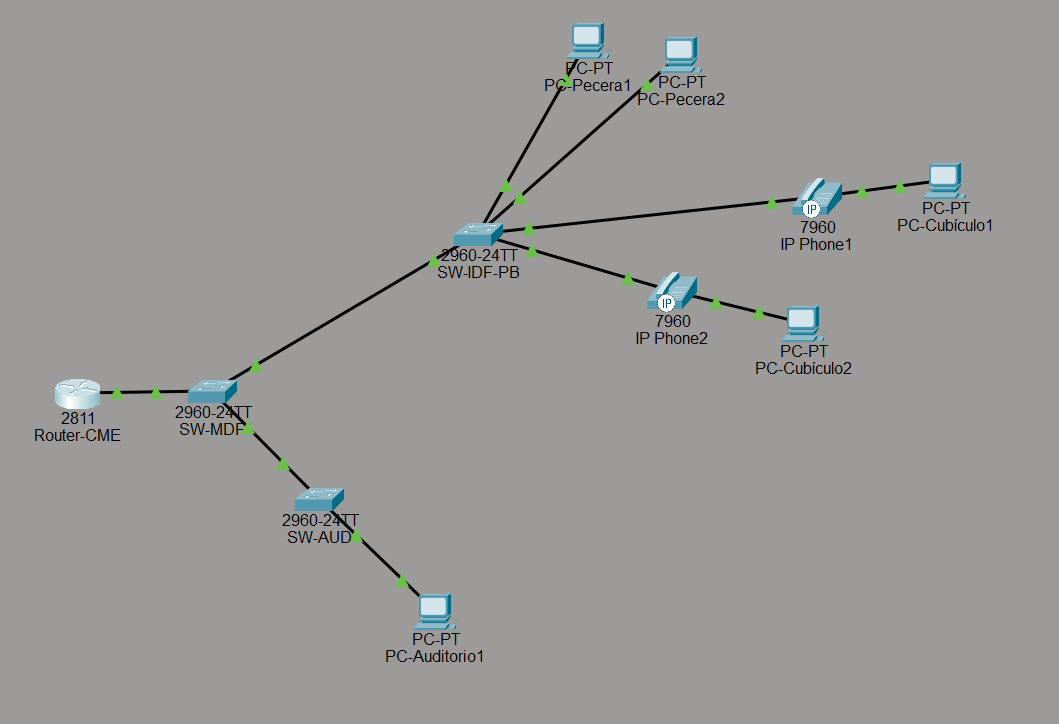
\includegraphics[width=\textwidth]{topo_principal.png}
    \caption{Topología lógica simulada -- Planta Baja Edificio Principal}
    \label{fig:topo_principal}
\end{figure}

La topología sigue una arquitectura jerárquica de tres niveles: el Router-CME actúa como núcleo lógico (inter-VLAN routing y servidor CME), el SW-MDF como switch core de distribución, y los switches SW-IDF-PB y SW-AUD como switches de acceso para cada zona. Los enlaces entre switches representan el backbone de fibra óptica Multimodo OM3 descrito en la cotización.

\begin{table}[h!]
\centering
\rowcolors{2}{GrisTabla}{white}
\renewcommand{\arraystretch}{1.3}
\begin{tabularx}{\textwidth}{@{} l l X @{}}
\toprule
\rowcolor{AzulUNAM!10}
\textbf{Dispositivo} & \textbf{Modelo PT} & \textbf{Rol} \\ \midrule
Router-CME & Cisco 2811 & Inter-VLAN Routing + Servidor CME (VoIP) \\
SW-MDF & Cisco 2960-24TT & Switch Core / MDF \\
SW-IDF-PB & Cisco 2960-24TT & Switch de Acceso / IDF Planta Baja \\
SW-AUD & Cisco 2960-24TT & Switch de Acceso / Auditorio \\
IP Phone 1, 2 & Cisco 7960 & Teléfonos IP (extensiones 1001 y 1002) \\
PC-Pecera 1, 2 & PC-PT & Zona Peceras (becarios) \\
PC-Cubículo 1, 2 & PC-PT & Zona Cubículos (conectadas en puente al teléfono) \\
PC-Auditorio1 & PC-PT & Zona Auditorio \\ \bottomrule
\end{tabularx}
\caption{Dispositivos modelados en la simulación -- Edificio Principal PB}
\end{table}

\subsection*{Esquema de Direccionamiento IP (VLSM)}

\begin{table}[h!]
\centering
\rowcolors{2}{GrisTabla}{white}
\renewcommand{\arraystretch}{1.3}
\begin{tabularx}{\textwidth}{@{} l l l l @{}}
\toprule
\rowcolor{AzulUNAM!10}
\textbf{VLAN} & \textbf{Nombre} & \textbf{Red} & \textbf{Gateway} \\ \midrule
VLAN 10 & Datos & 192.168.10.0/24 & 192.168.10.1 \\
VLAN 20 & Voz & 192.168.20.0/24 & 192.168.20.1 \\
VLAN 99 & Gestión & 192.168.99.0/24 & 192.168.99.254 \\ \bottomrule
\end{tabularx}
\caption{Esquema de direccionamiento por VLAN -- Edificio Principal PB}
\end{table}

\subsection*{Configuraciones Relevantes}

A continuación se presentan las configuraciones limpias de los dispositivos activos de la simulación.

\begin{tcolorbox}[enhanced, breakable, colback=black!95, colframe=AzulUNAM,
                  title=\textbf{SW-MDF -- Switch Core (MDF)}, arc=2mm, boxrule=1pt,
                  attach boxed title to top left={xshift=5mm, yshift=-3mm},
                  boxed title style={colback=AzulUNAM},
                  fontupper=\ttfamily\small\color{white}]
hostname SW-MDF\\
!\\
vlan 10 -- name Datos\\
vlan 20 -- name Voz\\
vlan 99 -- name Gestion\\
!\\
interface FastEthernet0/1\\
\hspace{1em}switchport mode trunk\\
\hspace{1em}switchport trunk allowed vlan 10,20,99\\
interface FastEthernet0/2\\
\hspace{1em}switchport mode trunk\\
\hspace{1em}switchport trunk allowed vlan 10,20,99\\
interface FastEthernet0/24\\
\hspace{1em}switchport mode trunk\\
\hspace{1em}switchport trunk allowed vlan 10,20,99\\
!\\
interface Vlan99\\
\hspace{1em}ip address 192.168.99.1 255.255.255.0
\end{tcolorbox}

\begin{tcolorbox}[enhanced, breakable, colback=black!95, colframe=AzulUNAM,
                  title=\textbf{SW-IDF-PB -- Switch de Acceso IDF Planta Baja}, arc=2mm, boxrule=1pt,
                  attach boxed title to top left={xshift=5mm, yshift=-3mm},
                  boxed title style={colback=AzulUNAM},
                  fontupper=\ttfamily\small\color{white}]
hostname SW-IDF-PB\\
!\\
interface FastEthernet0/1\\
\hspace{1em}switchport mode trunk\\
\hspace{1em}switchport trunk allowed vlan 10,20,99\\
interface FastEthernet0/2 -- 3  (Peceras, VLAN Datos)\\
\hspace{1em}switchport mode access\\
\hspace{1em}switchport access vlan 10\\
interface FastEthernet0/4 -- 5  (Telefonos IP, Voz + Datos)\\
\hspace{1em}switchport mode access\\
\hspace{1em}switchport access vlan 10\\
\hspace{1em}switchport voice vlan 20\\
\hspace{1em}mls qos trust cos
\end{tcolorbox}

\begin{tcolorbox}[enhanced, breakable, colback=black!95, colframe=AzulUNAM,
                  title=\textbf{Router-CME -- Inter-VLAN Routing y Servidor de Telefonía}, arc=2mm, boxrule=1pt,
                  attach boxed title to top left={xshift=5mm, yshift=-3mm},
                  boxed title style={colback=AzulUNAM},
                  fontupper=\ttfamily\small\color{white}]
hostname Router-CME\\
!\\
ip dhcp pool DATOS\\
\hspace{1em}network 192.168.10.0 255.255.255.0\\
\hspace{1em}default-router 192.168.10.1\\
ip dhcp pool VOZ\\
\hspace{1em}network 192.168.20.0 255.255.255.0\\
\hspace{1em}default-router 192.168.20.1\\
\hspace{1em}option 150 ip 192.168.20.1\\
!\\
interface FastEthernet0/0.10\\
\hspace{1em}encapsulation dot1Q 10\\
\hspace{1em}ip address 192.168.10.1 255.255.255.0\\
interface FastEthernet0/0.20\\
\hspace{1em}encapsulation dot1Q 20\\
\hspace{1em}ip address 192.168.20.1 255.255.255.0\\
!\\
telephony-service\\
\hspace{1em}max-ephones 5\\
\hspace{1em}max-dn 10\\
\hspace{1em}ip source-address 192.168.20.1 port 2000\\
\hspace{1em}auto assign 1 to 10\\
!\\
ephone-dn 1 -- number 1001\\
ephone-dn 2 -- number 1002
\end{tcolorbox}

\subsection*{Verificación de Conectividad}

Se realizaron pruebas de conectividad mediante comandos ICMP (ping) desde distintas zonas, confirmando el correcto funcionamiento del enrutamiento inter-VLAN y el backbone entre switches.

\begin{table}[h!]
\centering
\rowcolors{2}{GrisTabla}{white}
\renewcommand{\arraystretch}{1.3}
\begin{tabularx}{\textwidth}{@{} l l l l @{}}
\toprule
\rowcolor{AzulUNAM!10}
\textbf{Origen} & \textbf{Destino} & \textbf{IP Destino} & \textbf{Resultado} \\ \midrule
PC-Pecera1 & Gateway (Router-CME) & 192.168.10.1 & \textcolor{green!60!black}{\textbf{0\% pérdida}} \\
PC-Pecera1 & PC-Auditorio1 & 192.168.10.15 & \textcolor{green!60!black}{\textbf{0\% pérdida}} \\ \bottomrule
\end{tabularx}
\caption{Resultados de pruebas de conectividad ICMP -- Edificio Principal PB}
\end{table}

Los teléfonos IP Phone1 e IP Phone2 se registraron exitosamente en el servidor CME con las extensiones \textbf{1001} y \textbf{1002} respectivamente, obteniendo direcciones IP del pool de VLAN 20 (192.168.20.x) mediante DHCP.


% ================= SEPARADOR EDIFICIO ANEXO =================
\newpage
\vspace*{1cm}
\begin{tcolorbox}[enhanced, colback=OroUNAM, colframe=OroUNAM, arc=0mm, 
                  halign=center, valign=center, top=4mm, bottom=4mm]
    \LARGE\bfseries\color{white} FASE II: EDIFICIO ANEXO
\end{tcolorbox}
\addcontentsline{toc}{section}{Fase II: Edificio Anexo}
\vspace{0.5cm}

% Reseteamos los contadores
\setcounter{section}{7}
\setcounter{subsection}{0}

\subsection{Fenomenología Electromagnética y Normativa de Canalización}
Los medios de transmisión guiados sufren alteraciones electromagnéticas durante su recorrido, tales como atenuación, distorsión por retardo y diafonía (NEXT, FEXT). Para mitigar estas mermas en la banda ancha, el cableado UTP Categoría 6A utiliza un trenzado optimizado de 4 pares (23 AWG). La canalización debe respetar la norma ANSI/TIA-569-B, evitando el paralelismo cercano con líneas eléctricas de alta tensión y respetando las capacidades máximas de llenado para evitar tensiones mecánicas que degraden la certificación del enlace de 10 Gbps solicitado para las áreas del Edificio Anexo.

\subsection{Cálculo Analítico de Capacidad de Llenado para UTP Cat 6A}
De acuerdo con el análisis planimétrico de la Planta Baja del Edificio Anexo, se deben enrutar cables para proveer servicio a 65 nodos de red. Considerando la tasa de llenado sugerida (40\% al 60\%) para evitar deformaciones en la chaqueta del cable, y utilizando un diámetro estándar para UTP Categoría 6A, determinamos la capacidad en canaletas de PVC de $75 \text{ mm} \times 50 \text{ mm}$.

La capacidad máxima al 60\% de llenado es de 76 cables por canaleta. Por lo tanto, el cálculo analítico se expresa como:

\begin{equation}
\text{Número de canaletas} = \frac{65 \text{ cables}}{76 \text{ cables/canaleta}} \approx 0.85 \Rightarrow 1 \text{ canaleta principal}
\end{equation}

Para cubrir el recorrido principal, se utilizará una canaleta troncal asegurando que no se exceda el estrés físico sobre los conductores, permitiendo su despliegue hacia los cubículos y las "peceras" de becarios.

\section{Análisis Técnico y Cotización: Planta Baja}

\subsection{Cotización Desglosada: Cableado Estructurado (Cobre)}
Con base en los requerimientos, se necesitan 65 nodos de red en Categoría 6A marca Panduit configurados en T568 A/B para la Planta Baja del Edificio Anexo.

\begin{table}[h!]
\centering
\rowcolors{2}{GrisTabla}{white}
\renewcommand{\arraystretch}{1.3}
\begin{tabularx}{\textwidth}{@{} c X c c r @{}}
\toprule
\rowcolor{OroUNAM!20} % Color dorado sutil para diferenciar el anexo
\textbf{\#} & \textbf{Descripción Técnica} & \textbf{Cant.} & \textbf{P. Unit. (MXN)} & \textbf{Costo Total (MXN)} \\ \midrule
1 & Bobina UTP Panduit (CMR) 4 pares 23 AWG Cat 6A & 7 & \$ 8,500.00 & \$ 59,500.00 \\
2 & Jack Modular Mini-Com TX6A 10G RJ45 Cat 6A & 65 & \$ 150.00 & \$ 9,750.00 \\
3 & Patch Panel 48 puertos 1RU (Cargado) & 1 & \$ 4,500.00 & \$ 4,500.00 \\
4 & Patch Panel 24 puertos 1RU (Cargado) & 1 & \$ 2,800.00 & \$ 2,800.00 \\
5 & Faceplate (Placa y caja) Panduit 2 Módulos & 33 & \$ 100.00 & \$ 3,300.00 \\
6 & Patch Cord Cat 6A & 65 & \$ 150.00 & \$ 9,750.00 \\
7 & Organizadores (Frontal/Vertical Alta Densidad) & 4 & \$ 850.00 & \$ 3,400.00 \\
8 & Mano de Obra e Instalación (Misceláneos) & 1 & \$ 15,000.00 & \$ 15,000.00 \\ \midrule
\multicolumn{4}{r}{\textbf{Subtotal Cobre:}} & \textbf{\textcolor{AzulUNAM}{\$ 108,000.00}} \\ \bottomrule
\end{tabularx}
\end{table}

\subsection{Cotización Desglosada: Fibra Óptica (Backbone)}
El enlace de acometida y la conexión entre el MDF y el IDF de la Planta Baja se realizará con fibra óptica Multimodo OM3, cubriendo la interconexión con el Auditorio y el Site.

\begin{table}[h!]
\centering
\rowcolors{2}{GrisTabla}{white}
\renewcommand{\arraystretch}{1.3}
\begin{tabularx}{\textwidth}{@{} c X c c r @{}}
\toprule
\rowcolor{OroUNAM!20}
\textbf{\#} & \textbf{Descripción Técnica} & \textbf{Cant.} & \textbf{P. Unit.} & \textbf{Total (MXN)} \\ \midrule
1 & FO 6 hilos 50m, Multimodo 50/125µm (OM3) & 1 & \$ 6,000.00 & \$ 6,000.00 \\
2 & Conector Simplex Pre-pulido LC OptiCam MM & 12 & \$ 250.00 & \$ 3,000.00 \\
3 & Panel FAP Precargado 6 Acopladores Duplex LC & 1 & \$ 1,800.00 & \$ 1,800.00 \\
4 & Jumper FO Duplex LC-LC 3m (OM3/OM4) & 4 & \$ 800.00 & \$ 3,200.00 \\
5 & Módulos Transceptores Ópticos (GBIC/SFP 10G) & 8 & \$ 2,250.00 & \$ 18,000.00 \\ \midrule
\multicolumn{4}{r}{\textbf{Subtotal Fibra Óptica:}} & \textbf{\textcolor{AzulUNAM}{\$ 32,000.00}} \\ \bottomrule
\end{tabularx}
\end{table}

\section{Equipamiento Activo de Red y Servicios Convergentes}

\subsection{Conmutadores (Switches)}
Para soportar los 65 nodos de red (datos) más la telefonía convergente mediante Power over Ethernet (PoE) sin cableado adicional, la arquitectura se divide estratégicamente en el IDF PB y el Auditorio.

\begin{table}[h!]
\centering
\rowcolors{2}{GrisTabla}{white}
\renewcommand{\arraystretch}{1.3}
\begin{tabularx}{\textwidth}{@{} c X c r @{}}
\toprule
\rowcolor{OroUNAM!20}
\textbf{\#} & \textbf{Equipamiento Activo} & \textbf{Cant.} & \textbf{Total (MXN)} \\ \midrule
1 & Switch 48-port 10G PoE+ 390W, 4x10G SFP (IDF PB) & 1 & \$ 65,000.00 \\
2 & Switch 24 Ptos Base Line, 4x 10G SFP (Auditorio, No PoE) & 1 & \$ 22,000.00 \\ \midrule
\multicolumn{3}{r}{\textbf{Subtotal Equipamiento:}} & \textbf{\textcolor{AzulUNAM}{\$ 87,000.00}} \\ \bottomrule
\end{tabularx}
\end{table}

\subsection{Telefonía IP (Comunicaciones Unificadas)}
Se requieren 22 servicios de voz. Los teléfonos funcionarán en topología "puente-switch" conectando la PC y el teléfono a un solo nodo físico de la pared, alimentados por el Switch PoE+ del IDF.

\begin{table}[h!]
\centering
\rowcolors{2}{GrisTabla}{white}
\renewcommand{\arraystretch}{1.3}
\begin{tabularx}{\textwidth}{@{} c X c r @{}}
\toprule
\rowcolor{OroUNAM!20}
\textbf{\#} & \textbf{Dispositivos VoIP y Licenciamiento} & \textbf{Cant.} & \textbf{Total (MXN)} \\ \midrule
1 & Teléfonos IP SNOM D715 (Firmware ASTRA sin fuente) & 20 & \$ 38,000.00 \\
2 & Teléfonos IP Astra-Mitel 5370ip & 2 & \$ 6,000.00 \\
3 & Licencias Genéricas SIP Conmutador ASTRA R 5.4 & 22 & \$ 22,000.00 \\
4 & Licencias Propietarias IP Conmutador ASTRA R 5.4 & 2 & \$ 5,000.00 \\ \midrule
\multicolumn{3}{r}{\textbf{Subtotal Telefonía IP:}} & \textbf{\textcolor{AzulUNAM}{\$ 71,000.00}} \\ \bottomrule
\end{tabularx}
\end{table}

\section{Simulación de la Topología Lógica en Cisco Packet Tracer}

Al igual que en la Fase I, la simulación del Edificio Anexo se realizó como una síntesis representativa de las zonas principales de la Planta Baja. Los 65 nodos reales fueron abstraídos en dispositivos representativos por zona, permitiendo demostrar con claridad la segmentación lógica, el enrutamiento inter-VLAN, la telefonía IP y la conectividad hasta el Site de servidores.

\subsection*{Topología Implementada}

\begin{figure}[h!]
    \centering
    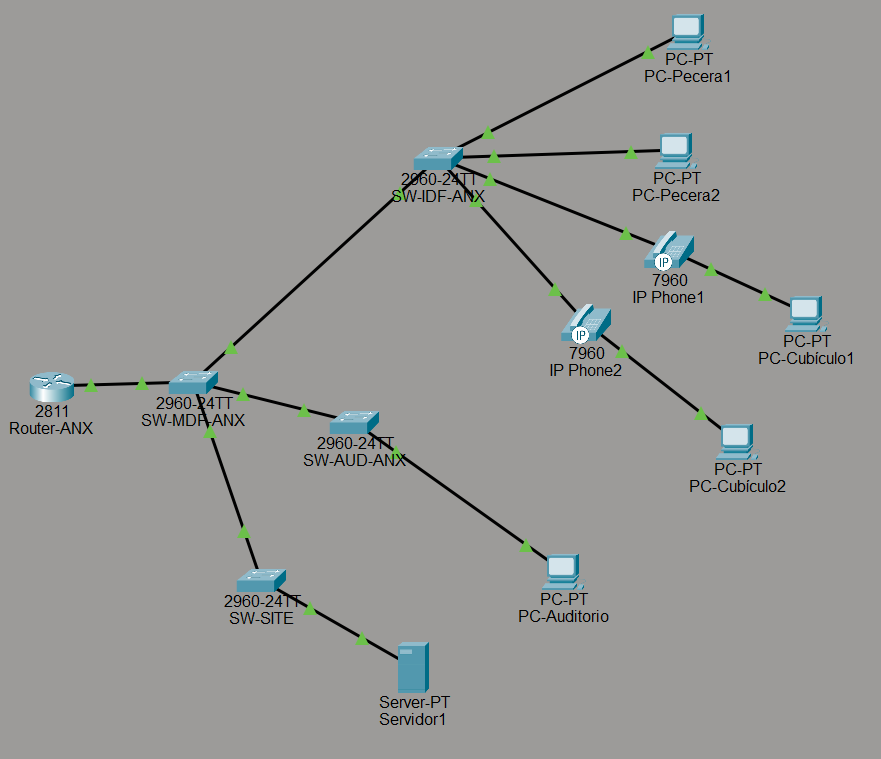
\includegraphics[width=\textwidth]{topo_anexo.png}
    \caption{Topología lógica simulada -- Planta Baja Edificio Anexo}
    \label{fig:topo_anexo}
\end{figure}

La topología del Anexo incorpora un elemento adicional respecto al Edificio Principal: el \textbf{SW-SITE}, que representa el cuarto de servidores conectado al MDF mediante enlace de fibra óptica. Esto refleja el requerimiento de conectividad hacia el Site descrito en las especificaciones del proyecto.

\begin{table}[h!]
\centering
\rowcolors{2}{GrisTabla}{white}
\renewcommand{\arraystretch}{1.3}
\begin{tabularx}{\textwidth}{@{} l l X @{}}
\toprule
\rowcolor{OroUNAM!20}
\textbf{Dispositivo} & \textbf{Modelo PT} & \textbf{Rol} \\ \midrule
Router-ANX & Cisco 2811 & Inter-VLAN Routing + Servidor CME (VoIP) \\
SW-MDF-ANX & Cisco 2960-24TT & Switch Core / MDF \\
SW-IDF-ANX & Cisco 2960-24TT & Switch de Acceso / IDF Planta Baja \\
SW-AUD-ANX & Cisco 2960-24TT & Switch de Acceso / Auditorio \\
SW-SITE & Cisco 2960-24TT & Switch de Acceso / Site Servidores \\
IP Phone 1, 2 & Cisco 7960 & Teléfonos IP (extensiones 2001 y 2002) \\
PC-Pecera 1, 2 & PC-PT & Zona Peceras (becarios) \\
PC-Cubículo 1, 2 & PC-PT & Zona Cubículos (conectadas en puente al teléfono) \\
PC-Auditorio & PC-PT & Zona Auditorio \\
Servidor1 & Server-PT & Servidor en Site (MDF) \\ \bottomrule
\end{tabularx}
\caption{Dispositivos modelados en la simulación -- Edificio Anexo PB}
\end{table}

\subsection*{Esquema de Direccionamiento IP (VLSM)}

\begin{table}[h!]
\centering
\rowcolors{2}{GrisTabla}{white}
\renewcommand{\arraystretch}{1.3}
\begin{tabularx}{\textwidth}{@{} l l l l @{}}
\toprule
\rowcolor{OroUNAM!20}
\textbf{VLAN} & \textbf{Nombre} & \textbf{Red} & \textbf{Gateway} \\ \midrule
VLAN 10 & Datos & 192.168.30.0/24 & 192.168.30.1 \\
VLAN 20 & Voz & 192.168.40.0/24 & 192.168.40.1 \\
VLAN 99 & Gestión & 192.168.99.0/24 & 192.168.99.254 \\ \bottomrule
\end{tabularx}
\caption{Esquema de direccionamiento por VLAN -- Edificio Anexo PB}
\end{table}

\subsection*{Configuraciones Relevantes}

\begin{tcolorbox}[enhanced, breakable, colback=black!95, colframe=OroUNAM,
                  title=\textbf{SW-MDF-ANX -- Switch Core (MDF)}, arc=2mm, boxrule=1pt,
                  attach boxed title to top left={xshift=5mm, yshift=-3mm},
                  boxed title style={colback=OroUNAM},
                  fontupper=\ttfamily\small\color{white}]
hostname SW-MDF-ANX\\
!\\
vlan 10 -- name Datos\\
vlan 20 -- name Voz\\
vlan 99 -- name Gestion\\
!\\
interface FastEthernet0/1  (hacia SW-IDF-ANX)\\
\hspace{1em}switchport mode trunk\\
\hspace{1em}switchport trunk allowed vlan 10,20,99\\
interface FastEthernet0/2  (hacia SW-AUD-ANX)\\
\hspace{1em}switchport mode trunk\\
\hspace{1em}switchport trunk allowed vlan 10,20,99\\
interface FastEthernet0/3  (hacia SW-SITE)\\
\hspace{1em}switchport mode trunk\\
\hspace{1em}switchport trunk allowed vlan 10,20,99\\
interface FastEthernet0/24  (hacia Router-ANX)\\
\hspace{1em}switchport mode trunk\\
\hspace{1em}switchport trunk allowed vlan 10,20,99\\
!\\
interface Vlan99\\
\hspace{1em}ip address 192.168.99.1 255.255.255.0
\end{tcolorbox}

\begin{tcolorbox}[enhanced, breakable, colback=black!95, colframe=OroUNAM,
                  title=\textbf{Router-ANX -- Inter-VLAN Routing y Servidor de Telefonía}, arc=2mm, boxrule=1pt,
                  attach boxed title to top left={xshift=5mm, yshift=-3mm},
                  boxed title style={colback=OroUNAM},
                  fontupper=\ttfamily\small\color{white}]
hostname Router-ANX\\
!\\
ip dhcp pool DATOS-ANX\\
\hspace{1em}network 192.168.30.0 255.255.255.0\\
\hspace{1em}default-router 192.168.30.1\\
ip dhcp pool VOZ-ANX\\
\hspace{1em}network 192.168.40.0 255.255.255.0\\
\hspace{1em}default-router 192.168.40.1\\
\hspace{1em}option 150 ip 192.168.40.1\\
!\\
interface FastEthernet0/0.10\\
\hspace{1em}encapsulation dot1Q 10\\
\hspace{1em}ip address 192.168.30.1 255.255.255.0\\
interface FastEthernet0/0.20\\
\hspace{1em}encapsulation dot1Q 20\\
\hspace{1em}ip address 192.168.40.1 255.255.255.0\\
!\\
telephony-service\\
\hspace{1em}max-ephones 5\\
\hspace{1em}max-dn 10\\
\hspace{1em}ip source-address 192.168.40.1 port 2000\\
\hspace{1em}auto assign 1 to 10\\
!\\
ephone-dn 1 -- number 2001\\
ephone-dn 2 -- number 2002
\end{tcolorbox}

\subsection*{Verificación de Conectividad}

\begin{table}[h!]
\centering
\rowcolors{2}{GrisTabla}{white}
\renewcommand{\arraystretch}{1.3}
\begin{tabularx}{\textwidth}{@{} l l l l @{}}
\toprule
\rowcolor{OroUNAM!20}
\textbf{Origen} & \textbf{Destino} & \textbf{IP Destino} & \textbf{Resultado} \\ \midrule
PC-Pecera1 & Gateway (Router-ANX) & 192.168.30.1 & \textcolor{green!60!black}{\textbf{0\% pérdida}} \\
PC-Pecera1 & Servidor1 (Site) & 192.168.30.16 & \textcolor{green!60!black}{\textbf{0\% pérdida}} \\
PC-Pecera1 & PC-Auditorio & 192.168.30.15 & \textcolor{green!60!black}{\textbf{0\% pérdida}} \\ \bottomrule
\end{tabularx}
\caption{Resultados de pruebas de conectividad ICMP -- Edificio Anexo PB}
\end{table}

Los teléfonos IP Phone1 e IP Phone2 se registraron exitosamente en el servidor CME con las extensiones \textbf{2001} y \textbf{2002} respectivamente, obteniendo direcciones IP del pool de VLAN 20 (192.168.40.x) mediante DHCP.

% ================= CONCLUSIONES Y REFERENCIAS =================
\vspace{1cm}
\begin{tcolorbox}[enhanced, colback=AzulUNAM, colframe=AzulUNAM, arc=0mm, 
                  halign=center, valign=center, top=4mm, bottom=4mm]
    \LARGE\bfseries\color{white} CIERRE DE PROYECTO
\end{tcolorbox}
\vspace{0.5cm}

\section{Conclusiones}
El proyecto de rediseño para el Instituto de Geografía de la UNAM cumple con los estándares vigentes en telecomunicaciones. La migración a Categoría 6A garantiza anchos de banda a futuro de hasta 10 Gbps, mientras que la integración del backbone en fibra OM3 de 6 hilos soporta altos niveles de redundancia. Al hacer uso de switches PoE+, se reducen radicalmente los costos de instalación paralela de energía para los teléfonos IP SNOM y Astra, maximizando la rentabilidad y logrando una infraestructura sumamente convergente, robusta y escalable tanto para el Edificio Principal como para el Edificio Anexo.

\section{Referencias}
\begin{itemize}
    \item ANSI/TIA/EIA-568-C.0, C.1, C.2: \textit{Estándares de Cableado de Telecomunicaciones en Edificios Comerciales (Cobre y Fibra Óptica).}
    \item ANSI/TIA/EIA-569-B: \textit{Estándar de Rutas y Espacios de Telecomunicaciones para Edificios Comerciales.}
    \item ANSI/TIA/EIA-606-A: \textit{Estándar de Administración para la Infraestructura de Telecomunicaciones.}
    \item Apuntes y Presentaciones de Clase: \textit{Redes de Datos Seguras, Facultad de Ingeniería, UNAM.}
\end{itemize}

\end{document}